%%
%% JSAI2026 Content - Merged Option (Maze + Transformer) - Revised v2
%% Changes from v1:
%%   - Improved figure captions with statistical details
%%   - Added Table 2 (Maze results) and Table 3 (F-regularization)
%%   - Condensed "Insight" section (removed Figure 7)
%%   - Clarified Table 1 FEP/MDL correspondence
%%

\title{
\jtitle{動的知識グラフの探索・統合を制御する統一ゲージの提案\\---\textit{Gauge what Knowledge Graph needs.}---}
\etitle{A Unified Gauge for Controlling Exploration and Integration in Dynamic Knowledge Graphs\\--- \textit{Gauge what Knowledge Graph needs.} ---}
}

\jaddress{{\small miyauchikazuyoshi@gmail.com}}

\author{%
\jname{宮内 和義\first}
\ename{Kazuyoshi Miyauchi}
}

\affiliate{
\jname{\first{}独立研究者}
\ename{Independent Researcher}
}

\begin{abstract}
Dynamic knowledge graphs face a fundamental ``When'' problem: when to accept new information as structure, and when to continue exploration. While existing approaches such as GraphRAG optimize \emph{what} to retrieve, they lack a principled criterion for \emph{when} to integrate. We propose \textbf{geDIG}, a unified gauge that operationally aligns the Free Energy Principle (FEP) and Minimum Description Length (MDL), quantifying this trade-off as $\F = \gednorm - \lambda(\Delta H_{\mathrm{norm}} + \gamma \Delta \mathrm{SP}_{\mathrm{rel}})$. We validate geDIG on two instantiations of dynamic knowledge graphs. (1) \textbf{Spatial KG (Maze)}: An agent building a cognitive map achieves 98\% success rate while rejecting 98\% of candidate edges. (2) \textbf{Semantic KG (Transformer)}: Attention matrices, viewed as token-relation graphs, exhibit a consistent transition from exploration to structure across layers ($p < 10^{-80}$), and F-regularization causally improves performance (+0.33pp, $p=0.038$). These results suggest geDIG as a general-purpose gauge for controlling when to explore and when to integrate in dynamic knowledge graphs.
\end{abstract}

\begin{document}
\begingroup
% jsaiac.sty renders the title block via tabular; default tabcolsep (=6pt)
% adds 12pt padding and can trigger Overfull \hbox warnings. Keep it local.
\setlength{\tabcolsep}{0pt}
\maketitle
\endgroup

%% ===========================================
\section{はじめに}
%% ===========================================

動的知識グラフ（Dynamic Knowledge Graph）において，新しい情報を「いつ」構造として受け入れ，「いつ」探索を続けるべきか——この\textbf{When問題}は未解決の基本課題である．
GraphRAG\cite{edge2024}やSelf-RAG\cite{asai2023}は「何を（What）」検索するかを最適化したが，「いつ（When）」統合するかはヒューリスティックに依存している．
本研究では，自由エネルギー原理（FEP）\cite{friston2010}と最小記述長（MDL）\cite{grunwald2007}を操作的に橋渡しする統一評価関数 \textbf{geDIG} (graph edit Distance and Information Gain) を提案し，この問題に原理的な解を与える．

geDIGの核心的仮説は，「\textbf{構造コストと伸展利得のトレードオフ}を単一スカラーで評価すれば，知識グラフの種類によらず，探索と統合を統一的に制御できる」というものである．
本稿では，この仮説を2種類の動的知識グラフで検証する：
\begin{itemize}
    \item \textbf{空間的KG（迷路）}：エージェントが構築する認知地図
    \item \textbf{意味的KG（Transformer）}：Attention行列が表現するトークン間関係グラフ
\end{itemize}
本稿の貢献は以下の3点である：
\begin{enumerate}
    \item 構造コストと伸展利得のトレードオフを単一スカラー化したgeDIGの定式化
    \item 2種類のKG（迷路・Transformer）における構造相転移の実証
    \item F正則化による因果的介入実験
\end{enumerate}

% NOTE: The page limit is strict (4 pages). Keep the conceptual illustration
% minimal; the AG/DG control-flow figure suffices for this version.

%% ===========================================
\section{geDIG：統一評価関数の定義}
%% ===========================================

geDIGは，「構造を変えるコスト」と「それによって得られる情報の質」の収支を単一スカラー $\F$ で評価する．

\begin{equation}
\F = \gednorm - \lambda \left( \Delta H_{\mathrm{norm}} + \gamma \cdot \Delta \mathrm{SP}_{\mathrm{rel}} \right)
\label{eq:gedig}
\end{equation}

ここで各項は以下に対応する（表\ref{tab:gedig_terms}）．
\begin{itemize}
\item $\gednorm$：正規化EPC (Edge Placement Cost)．グラフ編集距離（GED）の局所近似であり，MDLにおけるモデル記述長 $L(M)$ の増分に相当する．$\Delta$は比較対象間の差分（迷路：更新前後$G_{t-1},G_t$，Transformer：ランダムベースラインとの差）を表す．
\item $\Delta H_{\mathrm{norm}}$：シャノンエントロピーの差分（エントロピー増分；伸展利得, Extension Gain）．候補集合に対する重み付き分布$p$のエントロピー$H(p)$の変化として定義し，本稿では$\Delta H := H_{\mathrm{after}}-H_{\mathrm{before}}$（after-before）を採用する．$\Delta H>0$は候補分布の均質化（optionalityの増大）を表し，探索圧として$\F$を下げる（温度項）．
\item $\Delta \mathrm{SP}_{\mathrm{rel}}$：平均最短路長の相対短縮率．グラフ上のショートカット形成による効率化を表し，MDLにおけるデータ記述長 $L(D|M)$ の圧縮に相当する．
\end{itemize}

\paragraph{$\Delta\mathrm{EPC}_{\mathrm{norm}}$（$\gednorm$）の具体形}
再現性のため，本稿の実装で用いた局所GED近似を明記する．
更新前後のグラフ$G_{\mathrm{before}}=(V_b,E_b)$，$G_{\mathrm{after}}=(V_a,E_a)$に対し，編集操作はノード/エッジの挿入・削除のみとし，
\begin{equation}
\mathrm{GED}(G_b,G_a) := c_V\cdot \bigl||V_a|-|V_b|\bigr| + c_E\cdot \bigl(|E_b\setminus E_a|+|E_a\setminus E_b|\bigr)
\end{equation}
で近似する．これを正規化定数$C_{\max}$で割り，
\begin{equation}
\Delta\mathrm{EPC}_{\mathrm{norm}} \equiv \gednorm := \mathrm{GED}(G_b,G_a)/C_{\max}
\end{equation}
とする．迷路（検証I）では，クエリ近傍の$k$-hop局所部分グラフ上で評価し，$C_{\max}=c_V+c_E\max(1,|S_{\mathrm{link}}|)$（候補台固定）を用いた．
Attention（検証II）では$|V|$が系列長$L$で固定されるため，$c_V=0$かつ$C_{\max}=L^2$とすると$\gednorm$はエッジ密度$|E|/L^2$に一致する．

\paragraph{$\Delta \mathrm{SP}_{\mathrm{rel}}$の計算と計算量}
$\Delta \mathrm{SP}_{\mathrm{rel}}$は「近道」の寄与を測るため，平均最短路長$L(\cdot)$の相対短縮として
\begin{equation}
\Delta \mathrm{SP}_{\mathrm{rel}} := \max\!\left(0, \frac{L(G_{\mathrm{before}})-L(G_{\mathrm{after}})}{L(G_{\mathrm{before}})}\right)
\end{equation}
で定義する（$L(\cdot)$は最大連結成分上，または固定サンプルのノードペアに対する平均）．
迷路のmulti-hop評価（DG）では，全点対最短路（APSP）を毎回計算せず，固定ペア（既定400組）に対する距離をキャッシュし，追加エッジにより改善し得る距離のみをSSSPで増分更新することで計算量を抑えた．
Transformer解析では，層ごとのトークン関係グラフに対して同様の指標を算出し，スケール依存性を避けるためランダムベースラインからの差$\Delta\F$として解釈する．

候補集合に付与された重み$w_i$（類似度）から確率分布$p$を
\begin{equation}
p_i = \frac{w_i}{\sum_j w_j},\quad
H(p) = -\sum_i p_i \log p_i
\end{equation}
で定義し，正規化は$K=|S_{\mathrm{after}}|$として$\Delta H_{\mathrm{norm}} = (H_{\mathrm{after}}-H_{\mathrm{before}})/\log K$とする．

なお，$\F$の絶対値は正規化・グラフ化手続きに依存するため，異なるタスク間で直接比較しない．迷路では$\F$を最小化すべき目的関数（低いほど良い）として扱う一方，Transformer解析では同条件のランダム行列（Null仮説）からの差 $\Delta \F := \F-\F_{\mathrm{random}}$ を主要な解釈対象とし，$\F$がランダムベースラインより0に近い（高い）ほど「ランダムからの構造化」が進んでいると読む．

パラメータ $\lambda, \gamma$ は「情報温度」として機能し，構造の複雑さと情報の圧縮率のバランスを決定する．

\begin{table}[t]
\centering
\caption{geDIG構成項の理論的対応}
\label{tab:gedig_terms}
\scriptsize
\begin{tabular}{@{}lllll@{}}
\toprule
項 & 意味 & FEP & MDL & 役割 \\
\midrule
$\gednorm$ & 構造変更 & 複雑さ & $L(M)$増 & 抑制 \\
$\Delta H$ & 伸展利得（optionality） & 探索圧 & --- & 拡散 \\
$\Delta \mathrm{SP}$ & 経路短縮 & --- & $L(D|M)$圧縮 & 効率 \\
\bottomrule
\end{tabular}
\end{table}
\noindent\textbf{注記：}表\ref{tab:gedig_terms}のFEP/MDL対応は，本稿で扱うグラフ操作に対して「同型のトレードオフ構造」を与える操作的対応であり，厳密な上界・下界を与える形式的導出は今後の課題である．

\subsection{AG/DG 二段ゲート制御}
この $\F$ を用いて，エージェントは以下の2つのゲートを事象駆動的（Event-Driven）に制御する．
\begin{enumerate}
\item \textbf{AG (Attention Gate)}: 0-hop（直近）での評価．$g_0 = \F|_{\mathrm{local}} > \theta_{\mathrm{AG}}$ のとき，局所的な「違和感・未知」を検知し，探索モード（Exploration）を起動する．
\item \textbf{DG (Decision Gate)}: Multi-hop（数理推論）での評価．$g_{\min} = \min_h \F^{(h)} < \theta_{\mathrm{DG}}$ のとき，大域的な「近道・洞察」を発見したとみなし，統合モード（Integration）としてエッジを確定する．
\end{enumerate}
ここで$h$はDGにおけるルックアヘッド深さ（hop）であり，実装では候補エッジを貪欲に追加しながら$h=0,1,\dots,H$（最大$H=\texttt{max\_hops}$）の各段階で$g(h)$を計測し，その最小値を$g_{\min}$として用いる．

この機構により，システムは常に探索し続けるのではなく，「わからないときだけ調べ（AG）」，「わかったときだけ覚える（DG）」という自律的な振る舞いを獲得する（図\ref{fig:agdg_flow}）．

\begin{figure}[t]
\centering

\includegraphics[width=0.9\columnwidth]{figs/agdg_flow.pdf}
\caption{AG/DG制御フロー．観測$\to$候補生成$\to$AG評価（$g_0 > \theta_{\mathrm{AG}}$で探索継続）$\to$DG評価（$g_{\min} < \theta_{\mathrm{DG}}$でコミット）の事象駆動ループ．AGは局所的異常（高$\F$）を，DGは大域的効率化（低$\F$）を検知する．}
\label{fig:agdg_flow}
\end{figure}

%% ===========================================
\section{検証I：空間的KGとしての迷路探索}
%% ===========================================

\paragraph{KGとしての定式化}
部分観測迷路におけるエージェントの認知地図は，動的知識グラフの一形態である．
ノードは訪問した位置，エッジは移動可能な接続を表し，探索に伴いグラフが動的に成長する．
エージェントは周囲1マスしか見えないため，「見えた通路を全て記憶する」か「重要な分岐点のみ記憶する」かの選択を迫られる．

\paragraph{仮説}
geDIGのAG/DGゲートにより，エージェントは(1) 高い成功率を維持しつつ，(2) 候補エッジの大半を棄却する効率的な記憶構築が可能である．
すなわち，「いつ探索し，いつ構造化するか」をgeDIGが自律制御できる．

\paragraph{実験設定}
15$\times$15および25$\times$25の迷路を用いた．
具体的には，各候補行動（次セル）を位置・相対移動・通行可否・訪問回数・ゴール等からなる8次元特徴ベクトルで表し，クエリベクトルとの距離に基づく重み付き分布から$\F$を評価する．
パラメータは $\lambda=1.0, \gamma=1.0, \theta_{\mathrm{AG}}=0.4, \theta_{\mathrm{DG}}=0.0$，最大ステップ数は15$\times$15で250，25$\times$25で500とした．
比較対象として，(i) Random Walk（各ステップで可能行動から一様ランダムに選択し，直前の逆向きは回避），(ii) Greedy DFS（訪問済みセルを全保持し，未訪問近傍を優先するオンラインDFS），(iii) geDIGエージェントを設定した．
また，記憶効率の指標として圧縮率を定義する：各ステップで生成される候補エッジ総数$|E_{\mathrm{cand}}|$（観測近傍＋想起候補）を全て記憶する素朴方式に対し，DGでコミットしたエッジ総数$|E_{\mathrm{commit}}|$の棄却率 $1-|E_{\mathrm{commit}}|/|E_{\mathrm{cand}}|$ を圧縮率とした（geDIGのみ定義）．

\begin{figure}[h]
\centering
\begin{tabular}{l}
\toprule
\textbf{Algorithm 1} geDIG-driven Navigation \\
\midrule
1: \textbf{while} not at goal \textbf{do} \\
2: \quad $\mathbf{o}_t \leftarrow$ observe(neighbors) \\
3: \quad $g_0 \leftarrow \F(\mathcal{G}_t, \mathbf{o}_t)$ \quad // 0-hop evaluation \\
4: \quad \textbf{if} $g_0 > \theta_{\mathrm{AG}}$ \textbf{then} \quad // 違和感検知 \\
5: \quad \quad Expand search candidates \\
6: \quad \textbf{for} each candidate $c$ \textbf{do} \\
7: \quad \quad $g_{\min} \leftarrow \min_h \F^{(h)}(c)$ \quad // Multi-hop \\
8: \quad \quad \textbf{if} $g_{\min} < \theta_{\mathrm{DG}}$ \textbf{then} \quad // 近道発見 \\
9: \quad \quad \quad Update $\mathcal{G}_{t+1}$ with edge to $c$ \\
10: \quad Move to best direction \\
\bottomrule
\end{tabular}
\caption{geDIGによる自律探索アルゴリズム．AGが探索を，DGが構造化（エッジ追加）を制御する．}
\label{fig:algorithm}
\end{figure}


\subsection{結果：探索と統合の自律制御}
geDIGエージェントは，AG/DGのダイナミクスのみで迷路探索に成功した（表\ref{tab:maze_results}）．

\begin{table}[t]
\centering
\caption{迷路ナビゲーション結果（DFS迷路，部分観測）}
\label{tab:maze_results}
\small
\begin{tabular}{lccc}
\toprule
手法 & 成功率 & 平均ステップ & 圧縮率$^\dagger$ \\
\midrule
\multicolumn{4}{l}{\textbf{15$\times$15} ($n=100$, max\_steps=250)} \\
Random Walk & $0.75 \pm 0.08$ & $105.8 \pm 63.9$ & -- \\
Greedy DFS & $0.99 \pm 0.03$ & $82.1 \pm 30.8$ & -- \\
\textbf{geDIG} & $\mathbf{0.98 \pm 0.03}$ & $\mathbf{89.6 \pm 44.8}$ & \textbf{98\%} \\
\midrule
\multicolumn{4}{l}{\textbf{25$\times$25} ($n=60$, max\_steps=500)} \\
Random Walk & $0.40 \pm 0.12$ & $242.2 \pm 143.7$ & -- \\
Greedy DFS & $0.95 \pm 0.06$ & $242.2 \pm 106.9$ & -- \\
\textbf{geDIG} & $\mathbf{0.75 \pm 0.11}$ & $\mathbf{254.1 \pm 125.4}$ & \textbf{99\%} \\
\bottomrule
\multicolumn{4}{p{0.95\columnwidth}}{\scriptsize 成功率はWilson 95\% CIの半幅（$\pm$），平均ステップは成功エピソードのみの平均$\pm$標準偏差} \\
\multicolumn{4}{p{0.95\columnwidth}}{\scriptsize $^\dagger$圧縮率はgeDIGのみ定義：各ステップで生成される候補エッジ総数$|E_{\mathrm{cand}}|$を全て記憶する素朴方式と比べ，コミットしたエッジ$|E_{\mathrm{commit}}|$の棄却率として $1-|E_{\mathrm{commit}}|/|E_{\mathrm{cand}}|$} \\
\multicolumn{4}{p{0.95\columnwidth}}{\scriptsize geDIG vs Random Walk: 同一seedでの成功/失敗をペアにしたMcNemar検定（15$\times$15: $p < 10^{-5}$, 25$\times$25: $p < 0.001$）} \\
\end{tabular}
\end{table}

15$\times$15では，geDIGはRandom Walkを成功率・効率の両面で上回り，Greedy DFSと同等の成功率を維持しながら，候補エッジの大半を棄却する高い圧縮率（98\%）を達成した（図\ref{fig:maze_process}）．
25$\times$25では探索空間が拡大し成功率は低下するが，それでもRandom Walkより有意に高い成功率を示した．
これは，geDIGが「必要なトポロジー骨格」のみを選択的に記憶することを示す．
この構築されるグラフは，O'Keefeらが提唱した認知地図\cite{okeefe1978}や，認知科学におけるエピソード記憶の計算論的定義に対応する．
本モデルでは，AGが「驚き（未知）」を検知した地点をノードとし，DGが「理解（因果）」を確定した経路をエッジとして保存する．

\begin{figure}[t]
\centering
\begin{minipage}{0.48\columnwidth}
  \centering
  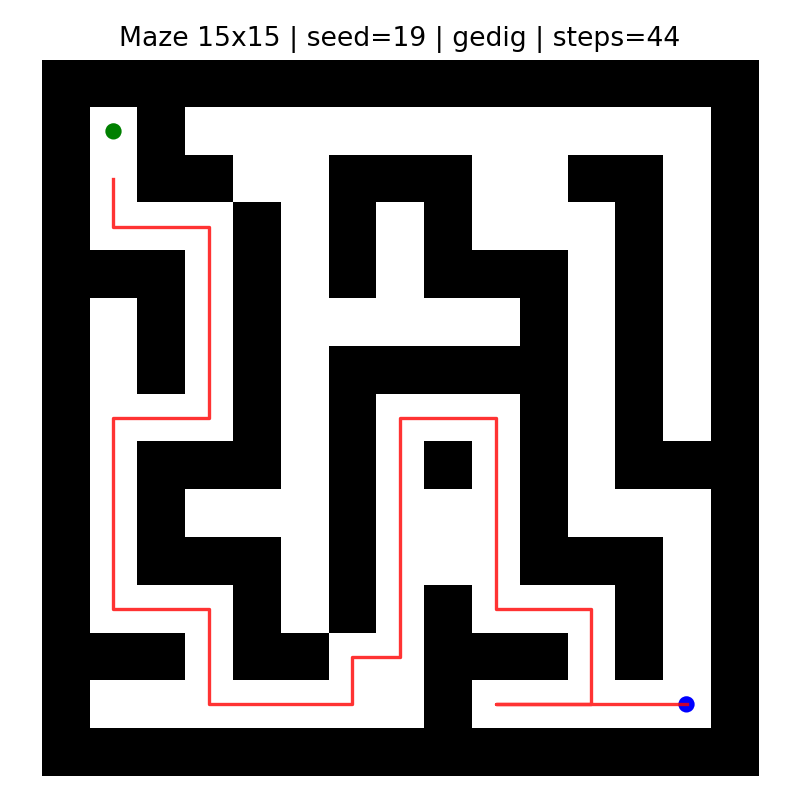
\includegraphics[width=\linewidth]{figs/maze_view.png}
  \centerline{(a) 実空間の探索軌跡}
\end{minipage}
\begin{minipage}{0.48\columnwidth}
  \centering
  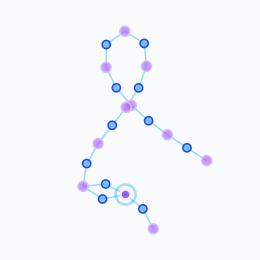
\includegraphics[width=0.9\linewidth]{figs/maze_graph_abstract.png}
  \centerline{(b) 抽象化された内部表現}
\end{minipage}
\caption{迷路探索における実空間と内部表現の対応．(a) 実際の迷路空間における探索軌跡．(b) geDIGが構築するエピソード記憶グラフの概念図．直線通路は圧縮され，分岐点（意思決定点，青）と経路（エッジ）のみが保持される．候補エッジに対するコミットエッジの棄却率（edge-compression）は98\%に達した．}
\label{fig:maze_process}
\end{figure}

%% ===========================================
\section{検証II：意味的KGとしてのTransformer}
%% ===========================================

\paragraph{KGとしての定式化}
TransformerのAttention行列$A_{ij}$は，トークン$i$からトークン$j$への「関係の強さ」を表す．
これを閾値処理（上位10\%）してグラフ化すると，動的に変化するトークン間関係グラフ——すなわち意味的KG——が得られる．
各層でこのグラフ構造が変化することは，情報の「探索」から「統合」への遷移を表している可能性がある．

\paragraph{仮説}
学習済みTransformerは，geDIG的な構造化を自発的に行っている．
具体的には，(1) 浅層では高エントロピーな探索状態（多様なトークン関係），(2) 深層では低エントロピーな構造状態（特定トークンへの集中）への相転移が観測されるはずである．
さらに，$\F$を直接最適化すれば性能が変化する（因果的証拠）．

\paragraph{実験設定}
対象モデルは BERT\cite{devlin2019}（12層）である．
SST-2（train）から短文200件を抽出し，各入力シーケンスを1サンプルとした．
各層の$\F$はヘッド平均のAttention行列から算出した（$\lambda=0.5, \gamma=0.5$, 系列長は最大128 token, 閾値は上位10\%）．
なお，本解析では$\F$の生値ではなく，完全ランダム（Null仮説）からの差$\Delta \F$（ベースラインからの乖離）を主要な解釈対象とする．これは閾値処理や系列長により$\F$の絶対スケールが変化し得るためである．
閾値は5\%〜20\%の範囲で変化させても同様の傾向が確認された．

\subsection{観測1：層別の構造相転移}
本稿でいう「相転移」は，臨界点や秩序変数の存在を主張するものではなく，層方向に沿った探索相$\to$構造相の\textbf{レジーム変化}を便宜上そう呼ぶ．
図\ref{fig:layer_f}にBERTの層別F値分布を示す．
学習済みモデルのAttention重みは，ランダム行列（同密度）に比べて$\F$が有意に高い値（0に近い）を示した（paired $t(199)=24.4$, $p < 10^{-60}$, $n=200$）．

さらに重要な発見は，深さ方向の推移である：
\begin{itemize}
    \item \textbf{Layer 0-1}: F値が低く（$\approx -0.50$），エントロピーが高い「探索相」．
    \item \textbf{Layer 4-5}: F値が上昇し（$\approx -0.45$），構造化が進む．
    \item \textbf{Layer 10-11}: 高い値で安定する「構造相」への相転移（$\approx -0.44$）．
\end{itemize}
Layer 0-1とLayer 10-11の差は統計的に有意である（paired $t(199)=32.6$, $p < 10^{-80}$, Cohen's $d=2.31$）．
この結果は，Transformerが層を重ねるごとに情報を「探索」から「結晶化」へと移行させていることを示唆する．

\begin{figure}[t]
\centering

\includegraphics[width=0.75\columnwidth]{figs/layer_wise_f.png}
\caption{BERTにおける層別F値の推移（SST-2, $n=200$文, ヘッド平均）．横軸は層番号，縦軸はF値（生の$\F$）．破線はランダム行列のベースラインであり，$\F$がベースラインより0に近い（高い）ほど「ランダムからの構造化」が進む．浅層（Layer 0-1）ではF値が低く高エントロピーな探索状態にあり，深層（Layer 10-11）ではF値が上昇し安定した構造化状態に収束する（Layer 0-1 vs 10-11: $p < 10^{-80}$）．}
\label{fig:layer_f}
\end{figure}

\subsection{観測2：ヘッドの機能分化}
同一層内でもヘッドごとにF値のばらつきが見られた．
一部のヘッドは極めて低いF値（拡散的で高エントロピー）を示し，他方は高いF値（集中した注意＝低エントロピー）を示した．
これはAttention Headが「探索担当」と「統合担当」のマルチエージェントとして機能分化していることを示唆する．

\subsection{観測3：F正則化による因果的介入}
以上の観測は相関関係に過ぎない．$\F$ が真に性能に関与しているなら，この値を直接最適化することで性能が変化するはずである．
DistilBERTを用いたSST-2タスクのFine-tuningにおいて，損失関数にF項による正則化を追加した：
$L_{\mathrm{total}} = L_{\mathrm{CE}} + \alpha \cdot \F$．
\paragraph{実装詳細（再現性）}
モデルは\texttt{distilbert-base-uncased}，SST-2（train 1000 / validation 500），最大長128，epoch=3，batch=16，AdamW（lr=$2\times10^{-5}$，weight\_decay=0.01）で学習した．
$\F$は\textbf{post-softmaxのAttention重み}から各層・各ヘッドで算出し，層平均を損失に加えた．
エッジ抽出の閾値処理は非微分なtop-$k$の代わりに，各ヘッドの90パーセンタイルを中心としたsigmoidによる\textbf{soft-threshold}（温度0.1）で近似し，密度（EPC）とエントロピーは微分可能に計算した．
$\Delta\mathrm{SP}_{\mathrm{rel}}$はsoft adjacencyの有限長（$\le4$）パワーに基づく到達度 proxy で近似した（閾値の勾配は安定化のため近似上固定）．

実験の結果（表\ref{tab:f_reg}），微弱な正則化（$\alpha=0.001$）でベースラインから有意に改善した（paired $t$-test, $p=0.038$, $n=3$ seeds）．
加えて，3/3 seedsで一貫した改善（+0.2〜0.4pp）が観測された．
一方で，過剰な正則化（$\alpha \geq 0.1$）は性能を悪化させた（表\ref{tab:f_reg}）．
この逆U字型の特性は，適切な「構造化圧」がモデルの汎化性能を引き出すことを因果的に示している．

注目すべきは，微弱な正則化（$\alpha=0.001$）でも有意な改善が見られた点である．
これは，学習済みTransformerが既に$\F$最小化に近い状態で動作していることを示唆する．
すなわち，Transformerは学習過程で自発的に構造化圧を獲得しており，geDIGはその「隠れた最適化目標」を顕在化したものと解釈できる．

\begin{table}[t]
\centering
\caption{F正則化の効果（SST-2, DistilBERT, $n=3$ seeds）}
\label{tab:f_reg}
\small
\begin{tabular}{lcc}
\toprule
$\alpha$ & Accuracy (\%, mean $\pm$ std) & $\Delta$ (pp) \\
\midrule
0 (Baseline) & 86.00 $\pm$ 0.53 & -- \\
0.001 & \textbf{86.33}$^*$ $\pm$ 0.46 & +0.33 \\
0.01 & 86.27 $\pm$ 0.70 & +0.27 \\
0.1 & 85.93 $\pm$ 1.10 & -0.07 \\
1.0 & 78.93 $\pm$ 1.55 & -7.07 \\
\bottomrule
\multicolumn{3}{l}{\scriptsize $^*$ paired $t$-test: $p=0.038$ vs Baseline（seed対応, $n=3$）} \\
\multicolumn{3}{l}{\scriptsize +0.33ppは誤り率を約2.4\%相対減（14.0\%$\to$13.7\%）} \\
\end{tabular}
\end{table}

% NOTE: Removed the alpha-sweep plot to satisfy the 4-page limit. The numeric
% result is fully reported in Table~\ref{tab:f_reg}.

%% ===========================================
\section{関連研究}
%% ===========================================
本研究の理論的基盤は，Fristonの自由エネルギー原理（FEP）\cite{friston2010}とGr\"{u}nwaldの最小記述長（MDL）\cite{grunwald2007}である．
両者は「複雑さと適合度のトレードオフ」という点で数学的に対応し\cite{tishby2000}，geDIGはこの対応をグラフ編集距離\cite{bunke1997}で操作可能にした．
また，GNN\cite{kipf2017}は確率的埋め込みでグラフを処理するが，geDIGは構造コストと情報利得を明示的に分離・統合する点で異なる．
認知地図の概念\cite{okeefe1978}は空間的KGとしての迷路実験の理論的背景を与える．

%% ===========================================
\section{考察とおわりに}
%% ===========================================

本研究では，2種類の動的KG——空間的KG（迷路）と意味的KG（Attention）——において，geDIG評価関数 $\F$ が共通の「構造化原理」として機能することを示した．
両者に共通するのは，高エントロピーな探索相から低エントロピーな構造相への相転移である：迷路では時間軸に沿って未知領域の拡張から経路の確定へ，Transformerでは層方向に沿ってLayer 0-1の多様なヘッド活性化からLayer 10-11の特定ヘッドへの集中へと遷移する．
F正則化実験により，この$\F$とモデル性能の因果関係を実証した．

\paragraph{geDIGと自由エネルギー}
geDIGの式 $\F = \gednorm - \lambda(\Delta H_{\mathrm{norm}} + \gamma \cdot \Delta \mathrm{SP}_{\mathrm{rel}})$ は，熱力学の自由エネルギー $F = E - TS$ と同型のトレードオフ構造を持つ：構造変更コスト$\gednorm$がエネルギー$E$に，伸展利得$\lambda \Delta H$が温度$\times$エントロピー$TS$に対応する．
この対応に基づけば，Transformerの層別$\F$推移は「高温（探索）から低温（構造化）への冷却過程」として解釈できる．
実際，Attention機構が入力情報の不確実性を減じ，意味的な近道を発見・固定化するダイナミクスは，熱力学的なアニーリング過程と整合する．

\paragraph{今後の展望}
geDIGの応用として，GraphRAG\cite{edge2024}やSelf-RAG\cite{asai2023}などの構造化RAGにおける「いつ検索し，いつ構造化するか」の自律制御が挙げられる．
現行のRAGは検索タイミングをヒューリスティックに決定しているが，geDIGのAG/DGゲートを導入することで，知識統合の意思決定を原理的に制御できる可能性がある．

%% ===========================================
%% 参考文献
%% ===========================================
\begin{thebibliography}{99}
\bibitem{friston2010} Friston, K.: The free-energy principle: a unified brain theory?, Nat. Rev. Neurosci., 11, 127--138 (2010).
\bibitem{grunwald2007} Gr\"{u}nwald, P.~D.: The Minimum Description Length Principle, MIT Press (2007).
\bibitem{vaswani2017} Vaswani, A., et al.: Attention Is All You Need, NeurIPS (2017).
\bibitem{gentner1983} Gentner, D.: Structure-mapping: A theoretical framework for analogy, Cognitive Science, 7(2), 155--170 (1983).
\bibitem{okeefe1978} O'Keefe, J., Nadel, L.: The Hippocampus as a Cognitive Map, Oxford University Press (1978).
\bibitem{bronstein2017} Bronstein, M. M., et al.: Geometric deep learning: going beyond euclidean data, IEEE Signal Processing Magazine, 34(4), 18--42 (2017).
\bibitem{devlin2019} Devlin, J., et al.: BERT: Pre-training of Deep Bidirectional Transformers for Language Understanding, NAACL (2019).
\bibitem{bunke1997} Bunke, H.: On a relation between graph edit distance and maximum common subgraph, Pattern Recognition Letters, 18(8), 689--694 (1997).
\bibitem{tishby2000} Tishby, N., et al.: The information bottleneck method, arXiv:physics/0004057 (2000).
\bibitem{edge2024} Edge, D., et al.: From Local to Global: A Graph RAG Approach to Query-Focused Summarization, arXiv:2404.16130 (2024).
\bibitem{asai2023} Asai, A., et al.: Self-RAG: Learning to Retrieve, Generate, and Critique through Self-Reflection, arXiv:2310.11511 (2023).
\bibitem{kipf2017} Kipf, T.~N., Welling, M.: Semi-Supervised Classification with Graph Convolutional Networks, ICLR (2017).

\end{thebibliography}

\end{document}
